\section{Conclusion}

\indent We studied how cooling devices reduce passenger discomfort in outdoor and semi-outdoor waiting areas. We estimated how much cooling reaches passengers, how much relief it provides, and which option performs best across the modeled weather conditions. We compared a fan and two evaporative coolers with a no-device baseline at 12 venues.

\indent In Model I, we found that the cooling at the outlet of an evaporative cooler is greater than the cooling in the waiting area after the air mixes. The amount of cooling available also depends on outdoor humidity. Model II used Standard Effective Temperature (SET) to compare how the devices feel to a passenger and how much discomfort each device reduces per kilowatt-hour. In Model III, the Large Evaporative Cooler led the comfort benchmark. The Fan led the minimax comparison for Grove Hall under the illustrative purchase, electricity, and water limits. Even with the Large Evaporative Cooler, peak-hour SET ranged from $28.12$ to $33.98\,^\circ\mathrm{C}$ and stayed above the $26\,^\circ\mathrm{C}$ comparison target at all 12 venues. Sensitivity analysis found five intervals where a Boston recommendation switched between the Fan and the Large Evaporative Cooler. In three of those intervals, increasing the outdoor temperature in the hot-humid scenario favored the Fan.

\indent The operating rule uses the $23$--$26\,^\circ\mathrm{C}$ band to decide when equipment can stay off. The equipment ranking uses hot-discomfort loss above the upper threshold.

\indent The modeled cases below show how hot-discomfort loss and available resources guide the operating choice.

\begin{table}[H]
  \centering
  \renewcommand{\arraystretch}{1.3}
  \begin{tabularx}{\textwidth}{>{\raggedright\arraybackslash}p{0.18\textwidth}Yp{0.48\textwidth}}
    \toprule
    \textbf{Option} & \textbf{When to use it} & \textbf{Evidence from the model} \\
    \midrule
    No cooling & The waiting area already meets the comfort target. & At Grove Hall in the hot-dry case, baseline SET is $24.44\,^{\circ}\mathrm{C}$, within the $23$--$26\,^{\circ}\mathrm{C}$ band. \\
    \rowcolor{gray!15}
    Fan & The Fan provides enough relief or cooling per kWh is the priority. & At Grove Hall in the hot-humid case, the Fan reduces SET from $27.66$ to $25.09\,^{\circ}\mathrm{C}$ using $0.25$ kWh and no water. \\
    Small Evaporative Cooler & Extra relief is needed and resources limit the choice. & At the Dallas bus shelter in peak heat, this cooler reduces SET by $0.40\,^{\circ}\mathrm{C}$ beyond the Fan, using an extra $0.95$ kWh and about $33$ kg of water. SET still exceeds the comfort target. \\
    \rowcolor{gray!15}
    Large Evaporative Cooler & Reducing remaining hot discomfort is the priority, and electricity and water are available. & This cooler leads the comfort benchmark at all 12 venues. At the Dallas bus shelter in peak heat, it improves on the Small Evaporative Cooler by $0.82\,^{\circ}\mathrm{C}$ SET using an extra $1.30$ kWh and about $45$ kg of water. \\
    \bottomrule
  \end{tabularx}
\end{table}

\indent The Grove Hall peak-hour comparison in Figure~\ref{fig:grove-hall-peak-tradeoff} shows why the operating choice depends on the value of the last increment of cooling. The Fan avoids $1.71$ SET degree-hours of hot discomfort using $0.25$ kWh. The Small Evaporative Cooler uses $1.20$ kWh and avoids only $1.22$ degree-hours, so the Fan outperforms it on both measures in this case. The Large Evaporative Cooler avoids $2.20$ degree-hours. Switching from the Fan to the Large Evaporative Cooler therefore buys about $0.49$ additional degree-hours of relief for $2.25$ extra kWh, and the modeled SET still exceeds the comfort target.

\begin{figure}[H]
    \centering
    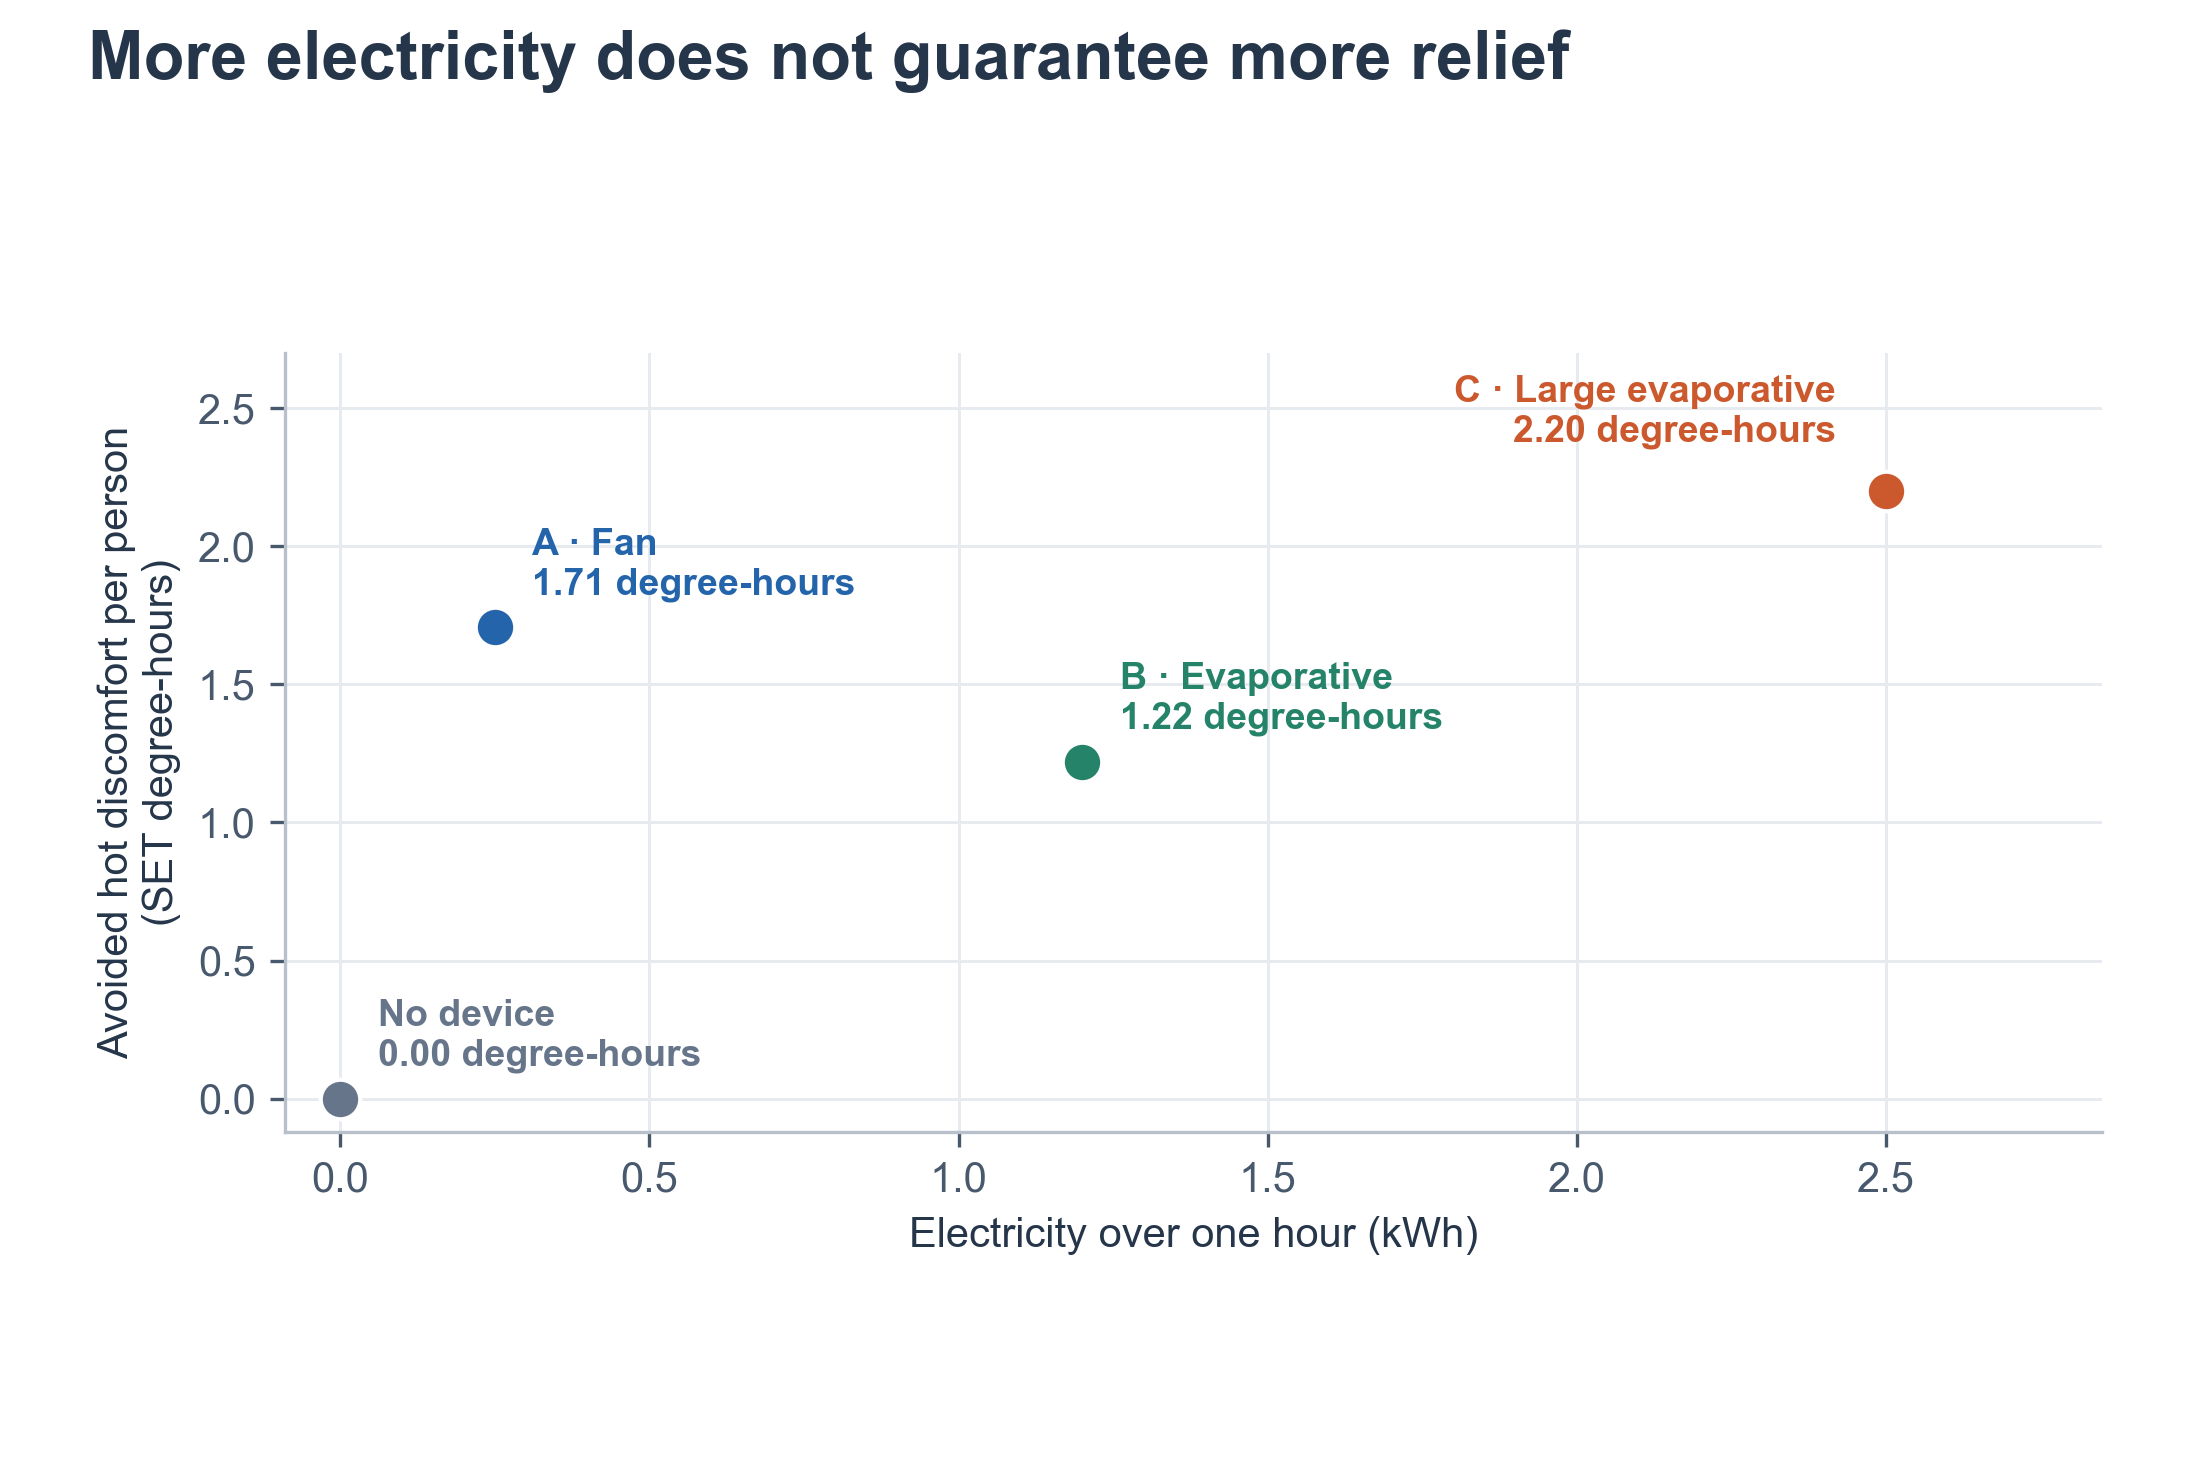
\includegraphics[width=0.66\linewidth,trim=0 0 0 76.32bp,clip]{Images/F2_boston_benefit_electricity.png}
    \caption{Electricity use and avoided hot discomfort at the Grove Hall bus shelter during the modeled peak-temperature hour.}
    \label{fig:grove-hall-peak-tradeoff}
\end{figure}

\indent Before installing equipment permanently, we recommend a pilot at Grove Hall. During humid heat and peak heat, measure air temperature, humidity, airspeed, and mean radiant temperature where passengers sit and stand. Compare the Fan and Large Evaporative Cooler at the same passenger positions, and test added shade during the peak period. The measurements would show where the Fan provides enough relief and whether shade helps close the gap to the comfort target.

\indent Across all 12 venues, we recommend the Large Evaporative Cooler when minimizing worst-case regret in hot-discomfort loss is the priority and the venue can meet its purchase, electricity, and water requirements. To identify fallback options, we recomputed regret with the Large Evaporative Cooler excluded and the remaining options feasible. In \textbf{Dallas}, choose the Small Evaporative Cooler at the bus shelter, rail platform, courtyard, and airport canopy when its resource requirements can be met. In \textbf{Boston}, choose the Fan at the bus shelter, rail platform, courtyard, and airport canopy. In \textbf{Phoenix}, choose the Small Evaporative Cooler at the rail platform and the Fan at the airport canopy. At the Phoenix bus shelter and courtyard, we recommend the Fan for its lower cost and water-free operation. The Small Evaporative Cooler has slightly lower maximum regret at those two sites, by less than $0.07$ SET degree-hours in each case. If water is unavailable for either cooler, use the Fan when cooling is needed and leave equipment off when the waiting area already meets the comfort target.
